%\documentclass[handout]{ximera}
\documentclass{ximera}

\usepackage{gensymb}
\usepackage{tabularx}
\usepackage{mdframed}
\usepackage{pdfpages}
%\usepackage{chngcntr}

\let\problem\relax
\let\endproblem\relax

\newcommand{\property}[2]{#1#2}




\newtheoremstyle{SlantTheorem}{\topsep}{\fill}%%% space between body and thm
 {\slshape}                      %%% Thm body font
 {}                              %%% Indent amount (empty = no indent)
 {\bfseries\sffamily}            %%% Thm head font
 {}                              %%% Punctuation after thm head
 {3ex}                           %%% Space after thm head
 {\thmname{#1}\thmnumber{ #2}\thmnote{ \bfseries(#3)}} %%% Thm head spec
\theoremstyle{SlantTheorem}
\newtheorem{problem}{Problem}[]

%\counterwithin*{problem}{section}



%%%%%%%%%%%%%%%%%%%%%%%%%%%%Jenny's code%%%%%%%%%%%%%%%%%%%%

%%% Solution environment
%\newenvironment{solution}{
%\ifhandout\setbox0\vbox\bgroup\else
%\begin{trivlist}\item[\hskip \labelsep\small\itshape\bfseries Solution\hspace{2ex}]
%\par\noindent\upshape\small
%\fi}
%{\ifhandout\egroup\else
%\end{trivlist}
%\fi}
%
%
%%% instructorIntro environment
%\ifhandout
%\newenvironment{instructorIntro}[1][false]%
%{%
%\def\givenatend{\boolean{#1}}\ifthenelse{\boolean{#1}}{\begin{trivlist}\item}{\setbox0\vbox\bgroup}{}
%}
%{%
%\ifthenelse{\givenatend}{\end{trivlist}}{\egroup}{}
%}
%\else
%\newenvironment{instructorIntro}[1][false]%
%{%
%  \ifthenelse{\boolean{#1}}{\begin{trivlist}\item[\hskip \labelsep\bfseries Instructor Notes:\hspace{2ex}]}
%{\begin{trivlist}\item[\hskip \labelsep\bfseries Instructor Notes:\hspace{2ex}]}
%{}
%}
%% %% line at the bottom} 
%{\end{trivlist}\par\addvspace{.5ex}\nobreak\noindent\hung} 
%\fi
%
%


\let\instructorNotes\relax
\let\endinstructorNotes\relax
%%% instructorNotes environment
\ifhandout
\newenvironment{instructorNotes}[1][false]%
{%
\def\givenatend{\boolean{#1}}\ifthenelse{\boolean{#1}}{\begin{trivlist}\item}{\setbox0\vbox\bgroup}{}
}
{%
\ifthenelse{\givenatend}{\end{trivlist}}{\egroup}{}
}
\else
\newenvironment{instructorNotes}[1][false]%
{%
  \ifthenelse{\boolean{#1}}{\begin{trivlist}\item[\hskip \labelsep\bfseries {\Large Instructor Notes: \\} \hspace{\textwidth} ]}
{\begin{trivlist}\item[\hskip \labelsep\bfseries {\Large Instructor Notes: \\} \hspace{\textwidth} ]}
{}
}
{\end{trivlist}}
\fi


%% Suggested Timing
\newcommand{\timing}[1]{{\bf Suggested Timing: \hspace{2ex}} #1}




\hypersetup{
    colorlinks=true,       % false: boxed links; true: colored links
    linkcolor=blue,          % color of internal links (change box color with linkbordercolor)
    citecolor=green,        % color of links to bibliography
    filecolor=magenta,      % color of file links
    urlcolor=cyan           % color of external links
}

\title{Similarities}
\author{Bart Snapp and Brad Findell}

\outcome{Learning outcome goes here.}

\begin{document}
\begin{abstract}
Abstract goes here.  
\end{abstract}
\maketitle

\begin{teachingnote}
Precede this with the Connected Math Program's stretching activity, which doesn't take a whole class.  
Supplies:  rubber bands, extra paper, tape.   
In the examples, include some pairs that are not similar.  Somehow require that they actually do the zooming.  Actually measure from eye to plastic bag and from eye paper to find the scale factor.  Use string for the measuring.  Use a sighting activity to the board.
\end{teachingnote}

\begin{problem}
Based on your experience with the stretching activity, write a definition of dilation.  Be sure to indicate (1) what it takes to specify the transformation, and (2) how to produce the image of a given point.  
\vspace{0.6in}
\end{problem}

\begin{problem}
Based on your experience with the stretching activity, describe for a dilation: 
\begin{enumerate}
\item What happens to line segments? 
\vspace{0.2in}
\item What happens to angles?  
\vspace{0.2in}
\item What happens to lines passing through the center of the dilation?
\vspace{0.2in}
\item What happens to lines not passing through the center of the dilation?
\vspace{0.2in}
\end{enumerate}
\end{problem}

%Every dilation has the following properties:
%\begin{enumerate}[(i)]
%\item It maps lines to lines, rays to rays, and segments to segments.
%\item It changes distance by a factor of $r$, where $r$ is the scale factor of the dilation.
%\item It maps every line passing through the center of dilation to itself, and it maps every line not passing through the center of the dilation to a parallel line.  
%\item It preserves angle measure.
%\end{enumerate}

\begin{definition}
A geometric figure is \emph{simliar} to another if the second can be obtained from the first by a sequence of rotations, reflections, translations, and dilations.  
\end{definition}

\begin{problem}
For each of the pairs of objects on the following pages, do the following:  
\begin{enumerate}
\item Trace the smaller figure on plastic.  Then close one eye and try to hold the plastic between your eye and the paper so that the tracing ``exactly'' covers the larger figure.   Be sure that the plane of the paper and the plane of the plastic are parallel.  (Why does this matter?) 
\item If the objects are similar, find a sequence of rotations, reflections, translations, and dilations that takes one figure onto the other.  
\item If the objects are similar, try to find a single dilation that demonstrates the similarity.   If you cannot find such a dilation, explain how you know you cannot.  
\end{enumerate}
\end{problem}
\vfill

\begin{image}
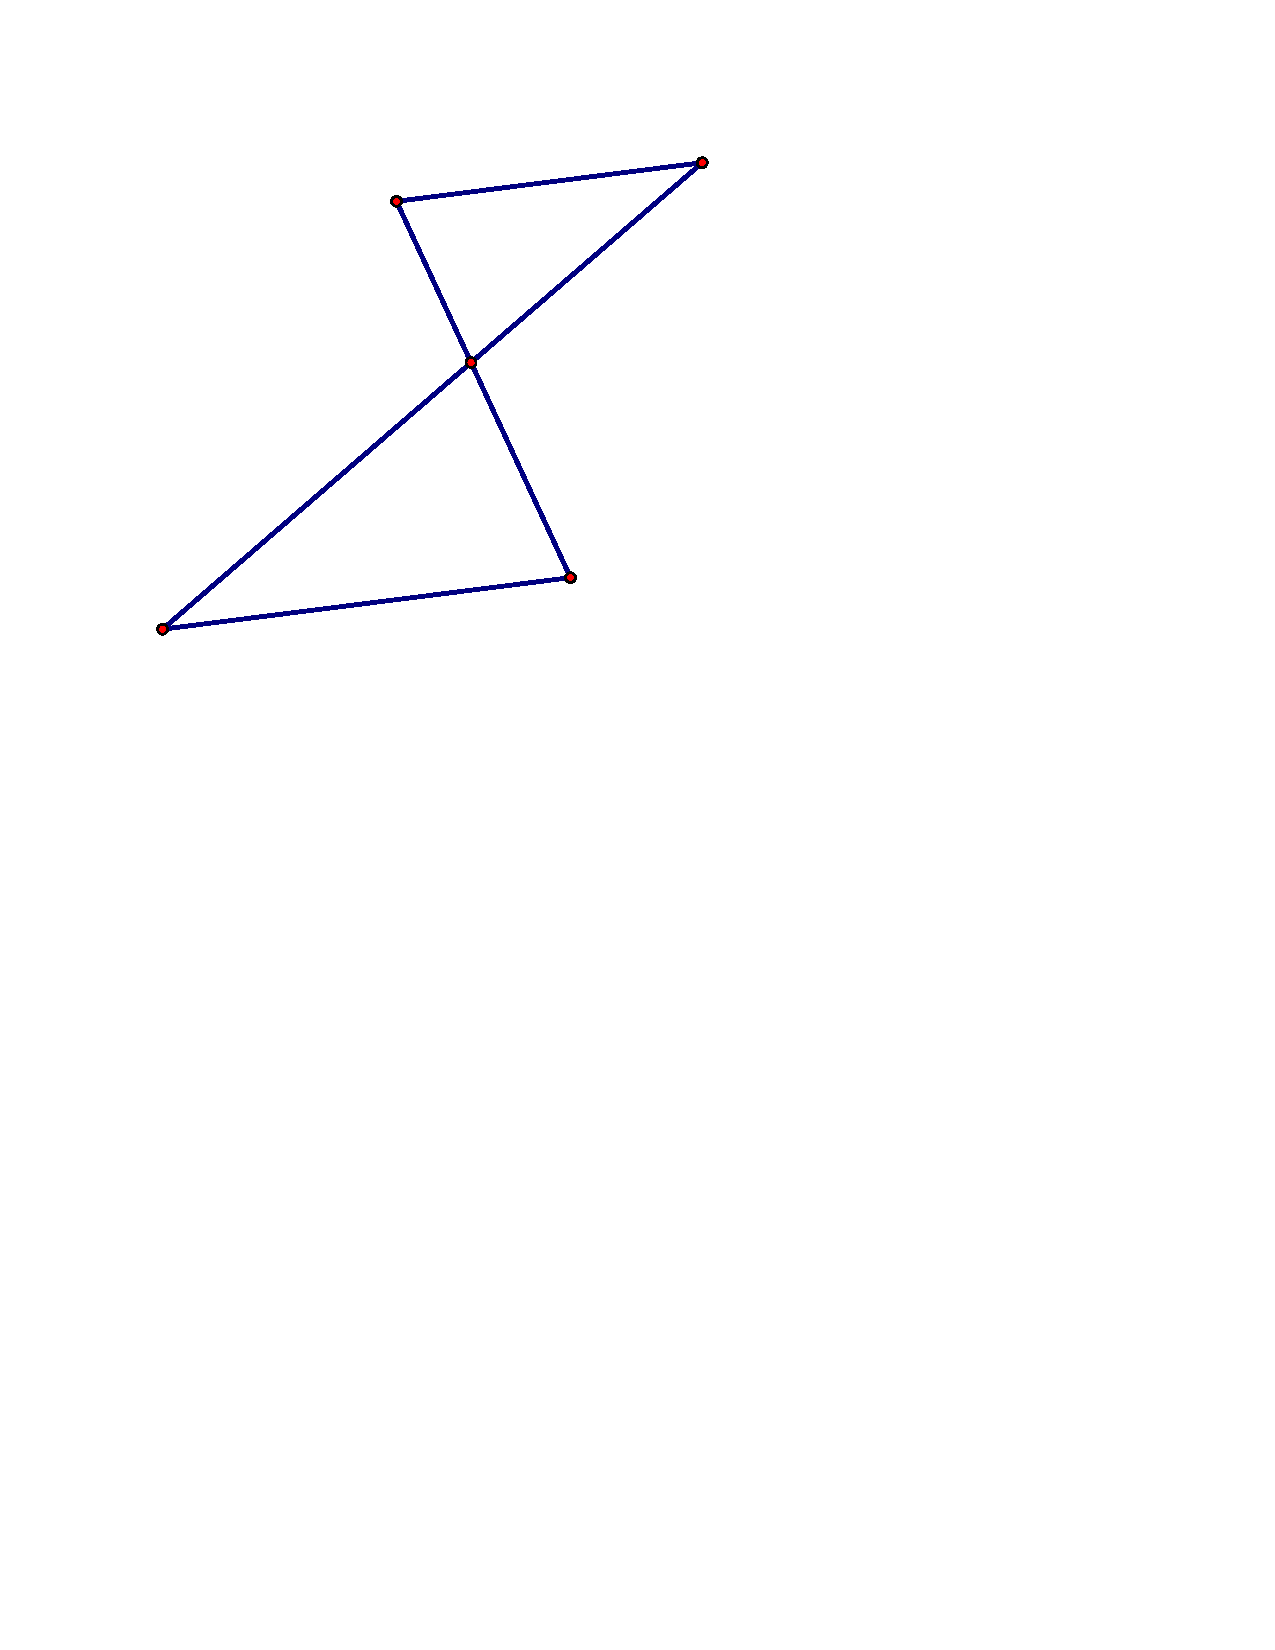
\includegraphics{similarTriangles1}
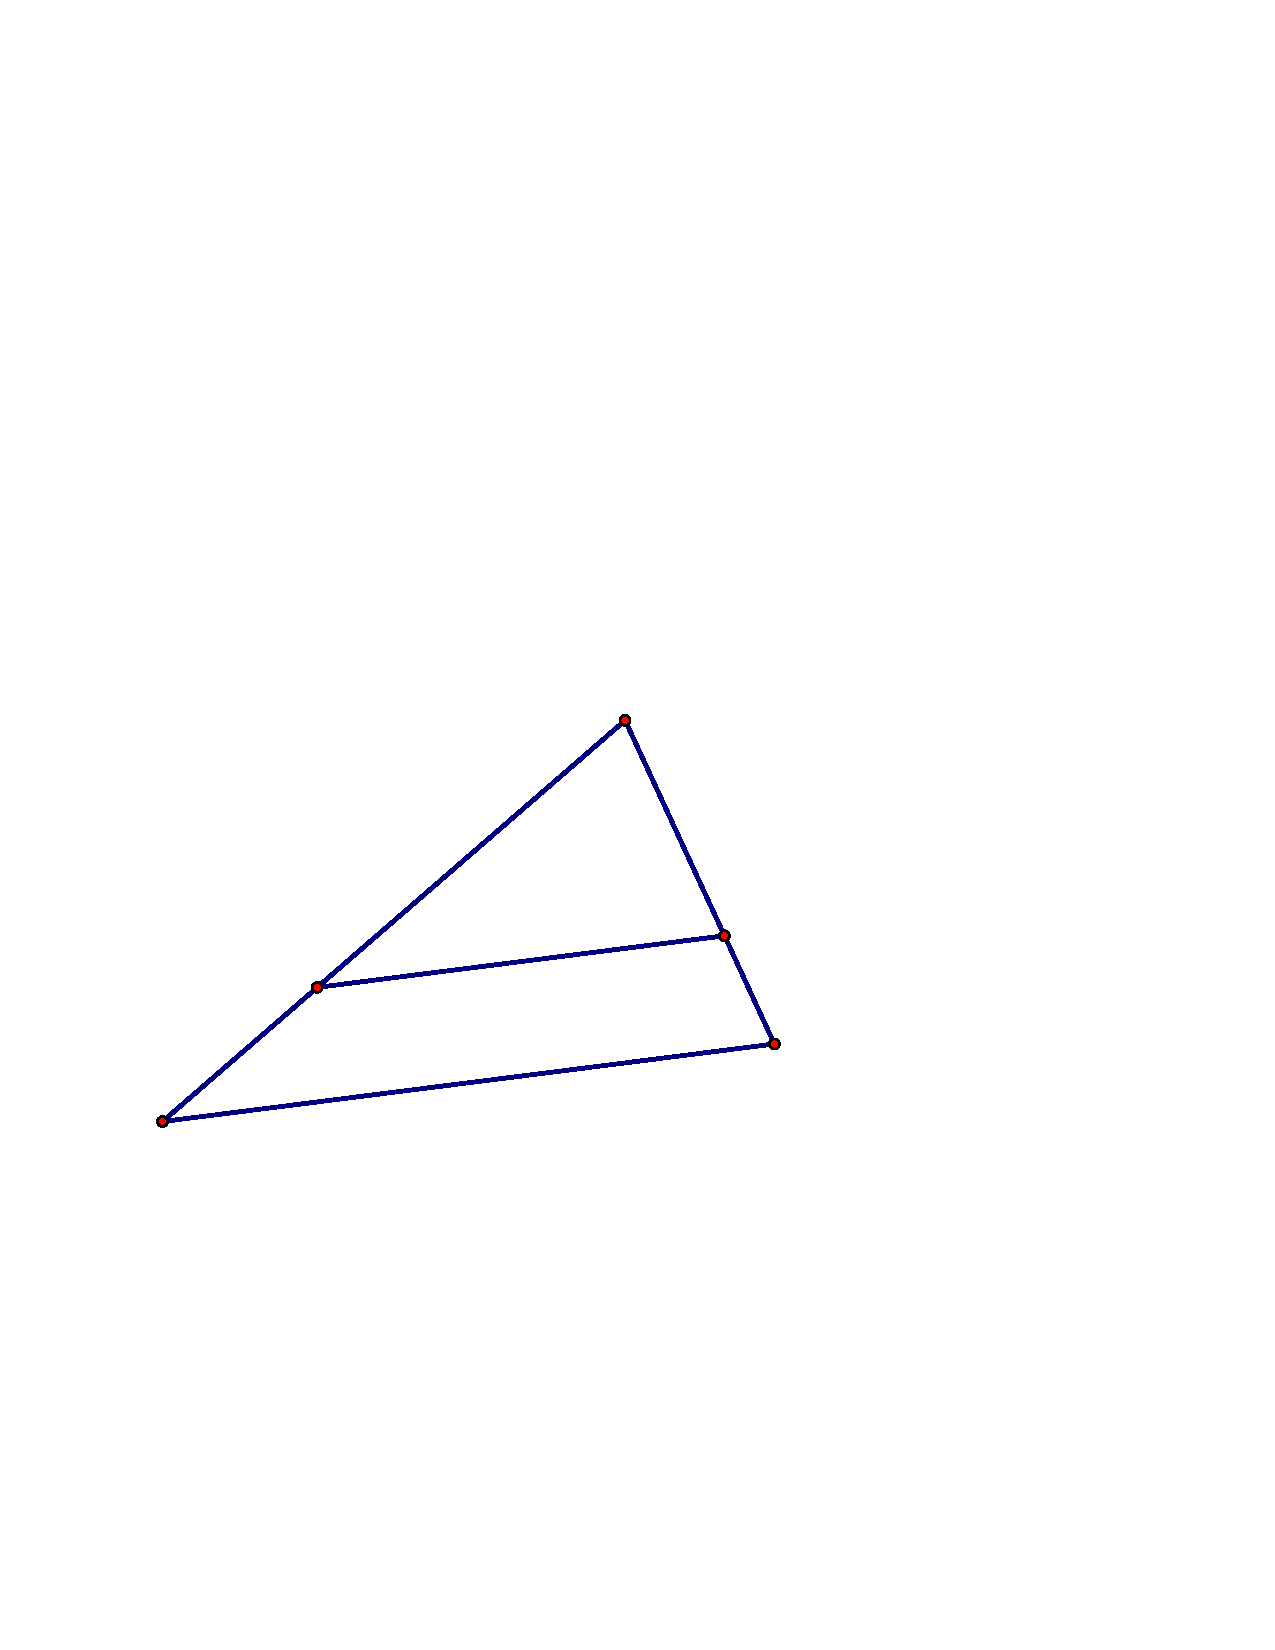
\includegraphics{similarTriangles2}
\end{image}

\vfill
\newpage
\vfill
\begin{image}
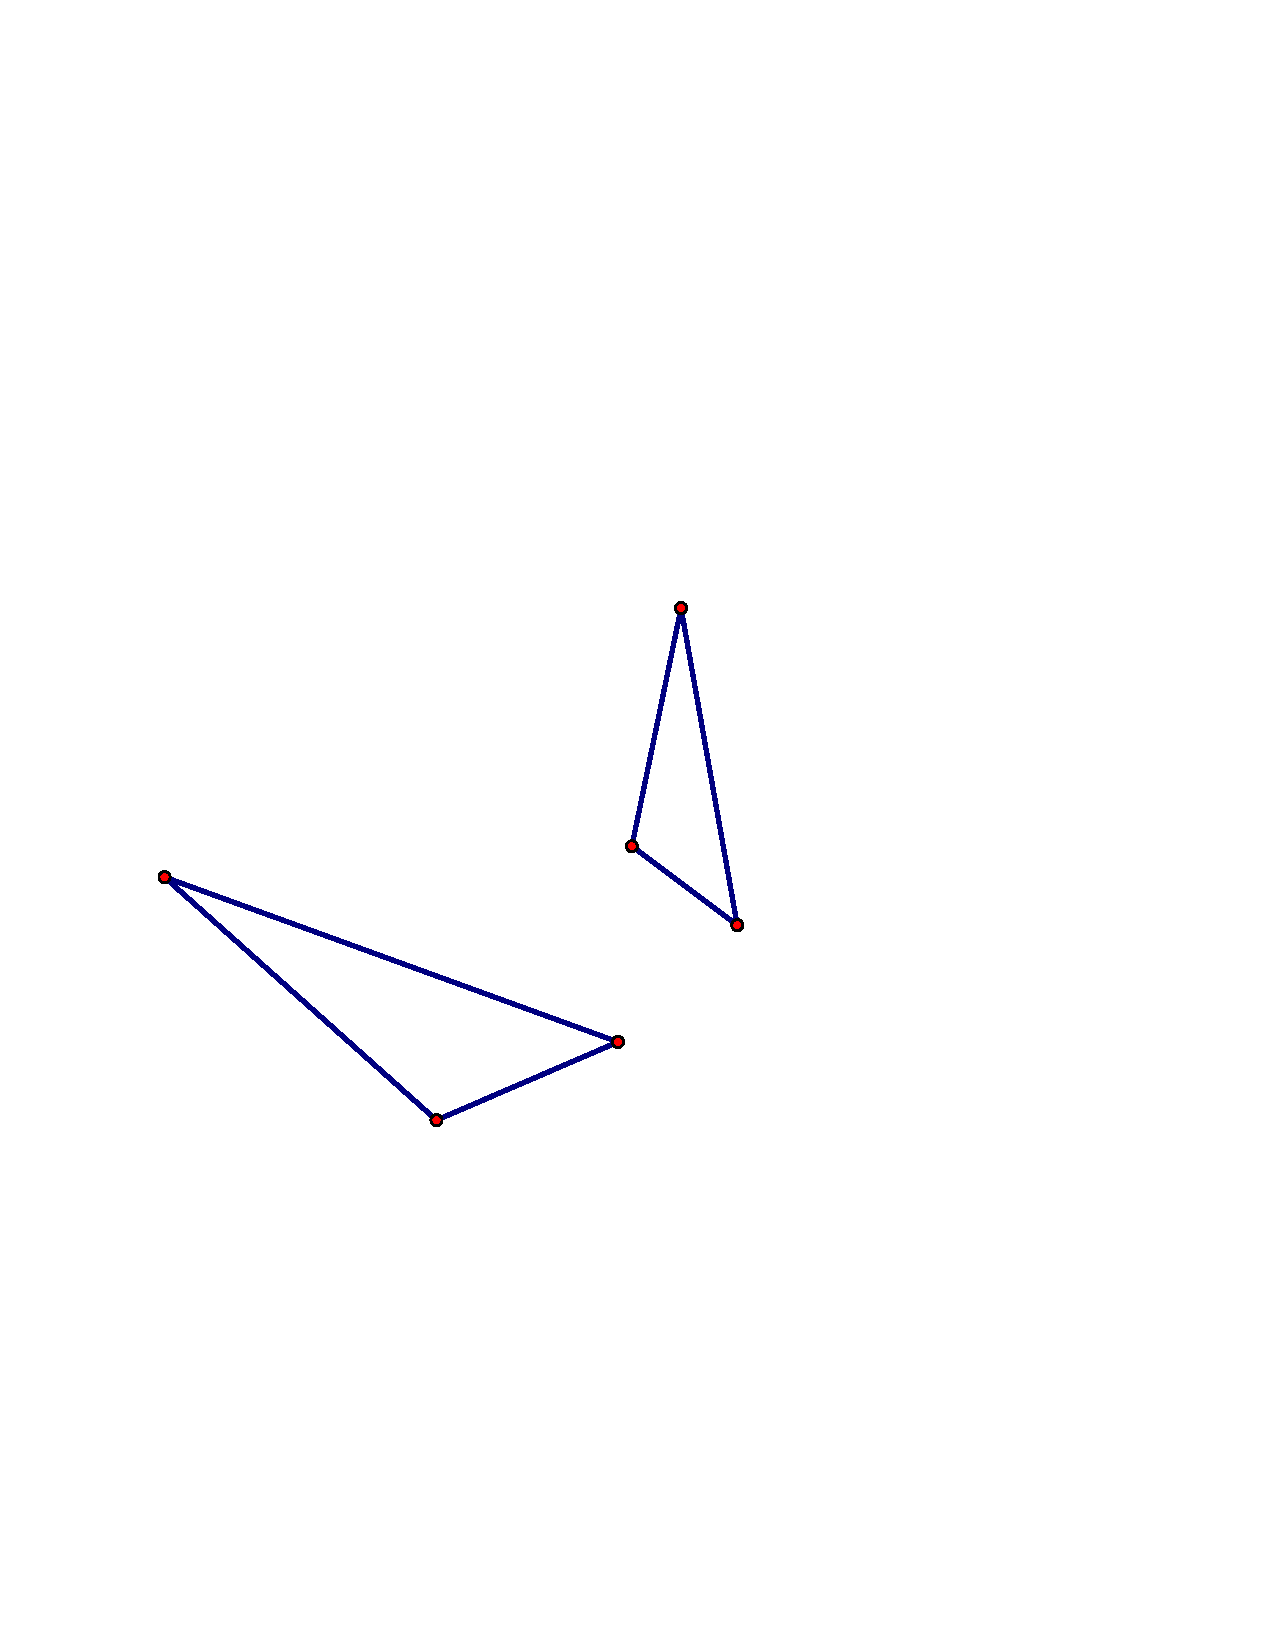
\includegraphics{similarTriangles3}
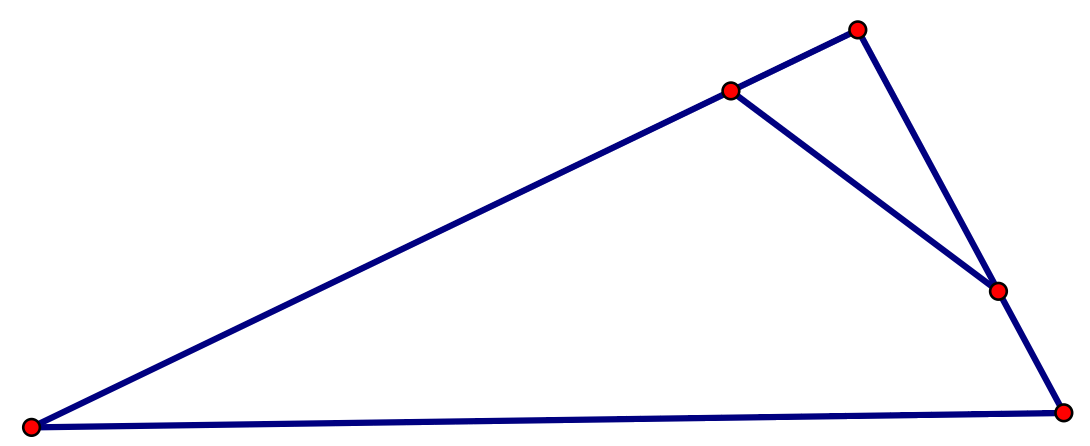
\includegraphics[scale=0.6]{similarTriangles5}
\end{image}
\vfill
\newpage
\begin{problem}
Describe a general (and foolproof) way of demonstrating that any two circles are 
similar.%\standardhs{G-C.1} 
\fixnote{Cite G-C.1}
\end{problem}
\vfill
\begin{image}
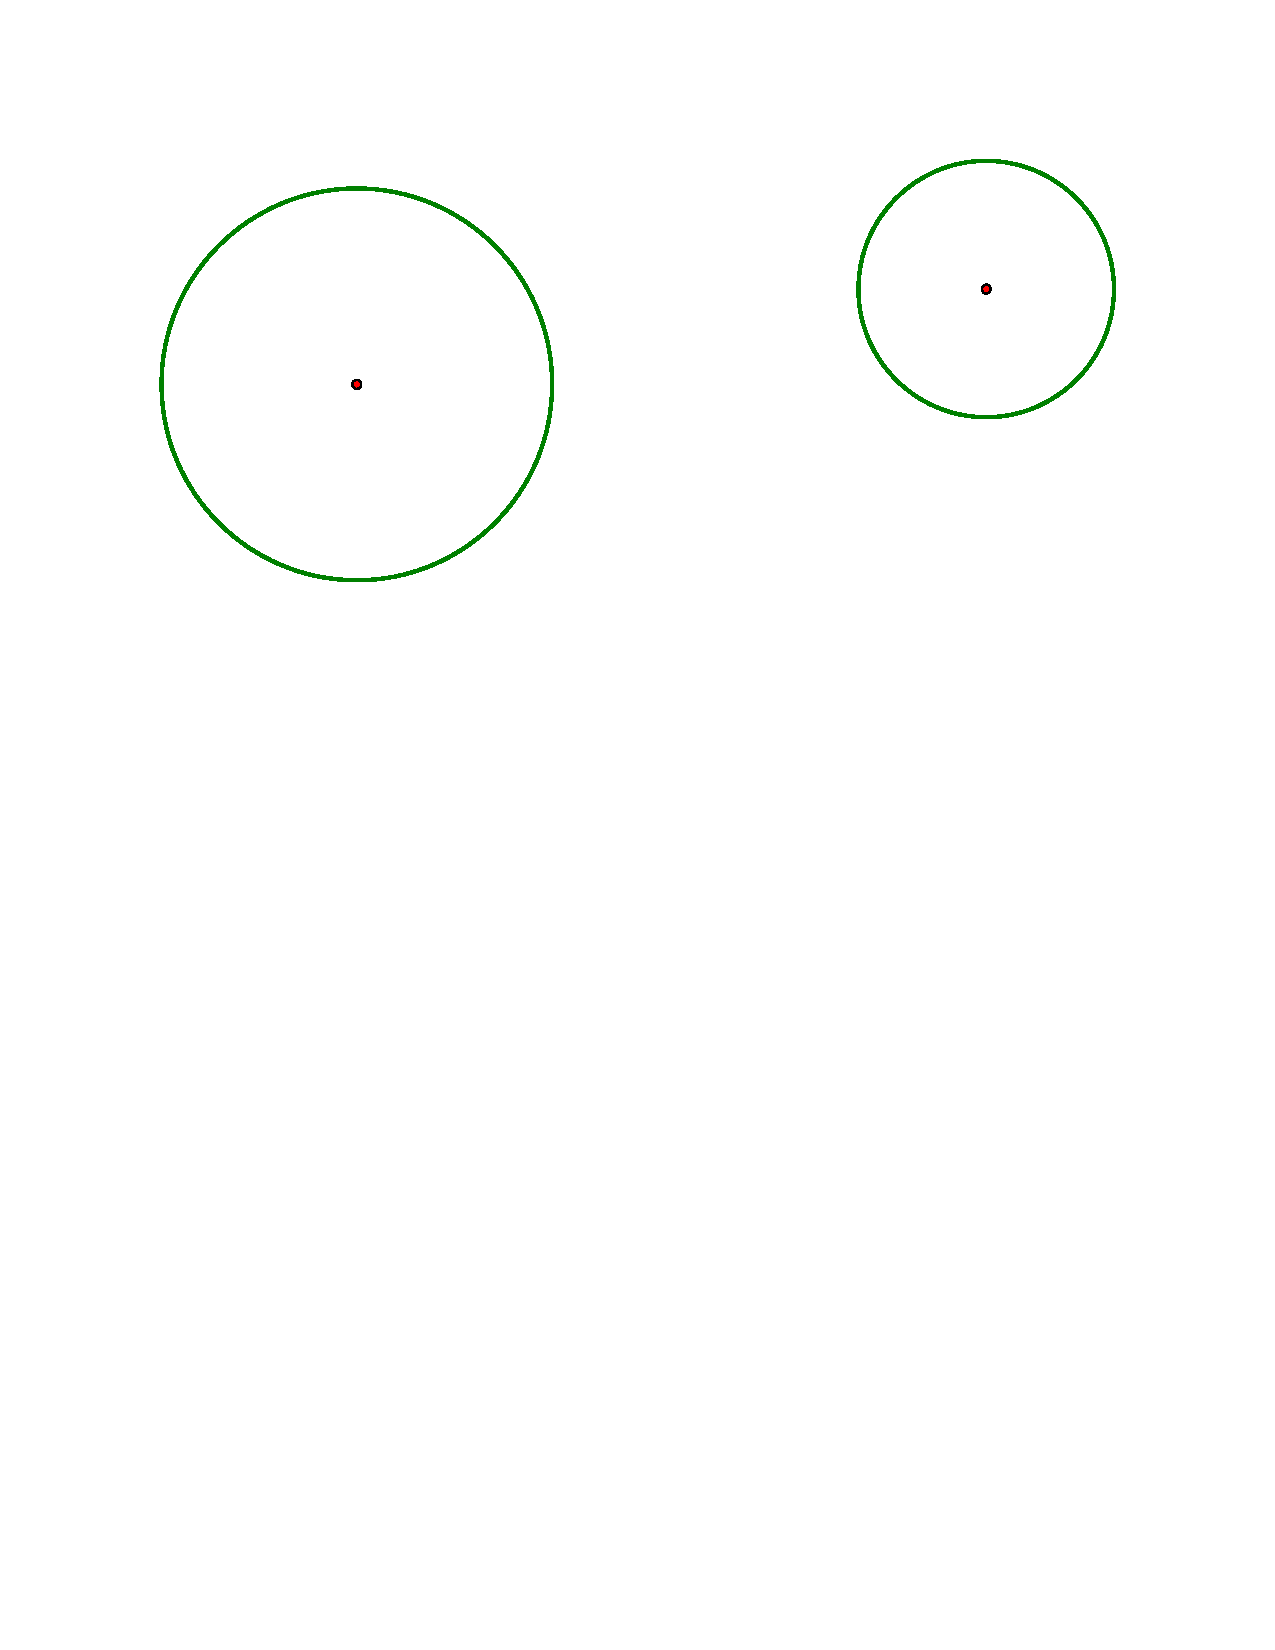
\includegraphics{similarCircles1}
\end{image}
\vfill
\newpage

\begin{problem}
Describe a general (and foolproof) way of demonstrating that any two parabolas are similar. 
\end{problem}
\vfill
\begin{image}
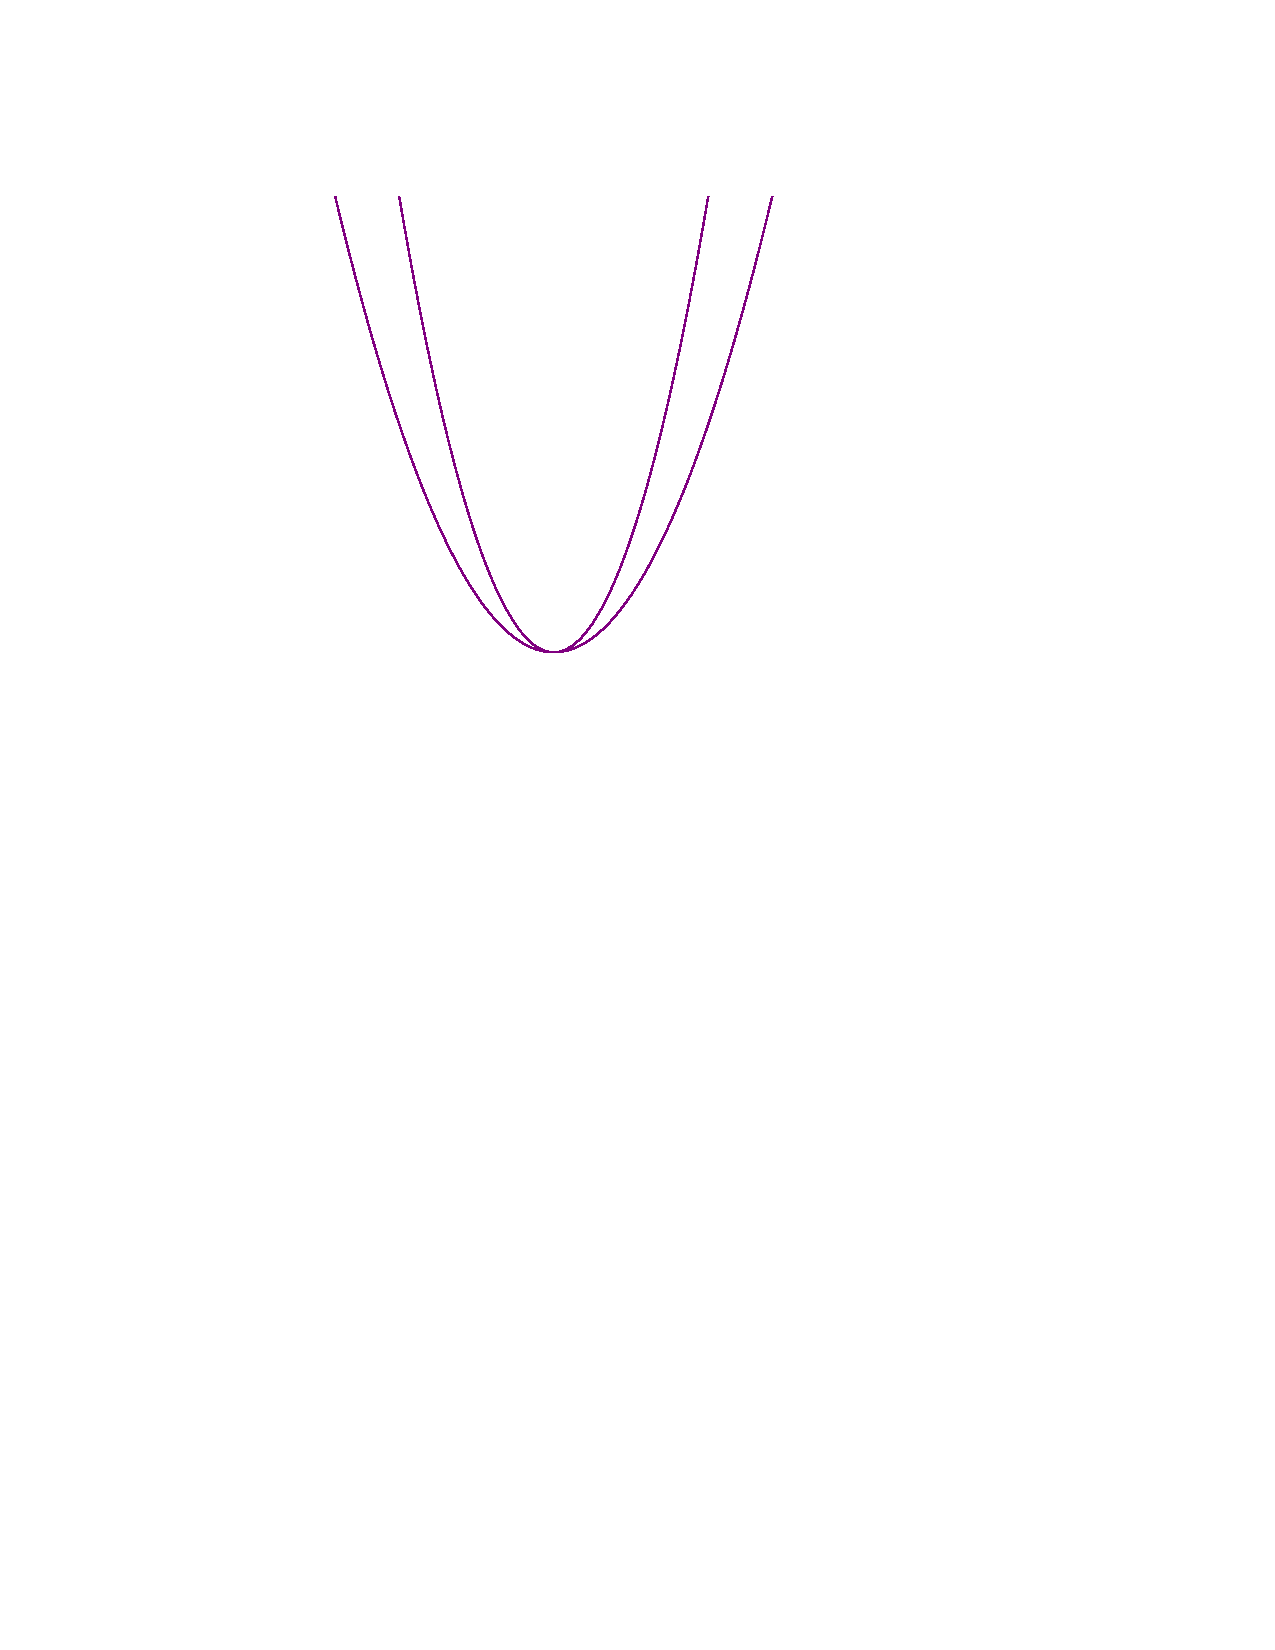
\includegraphics{similarParabolas1}
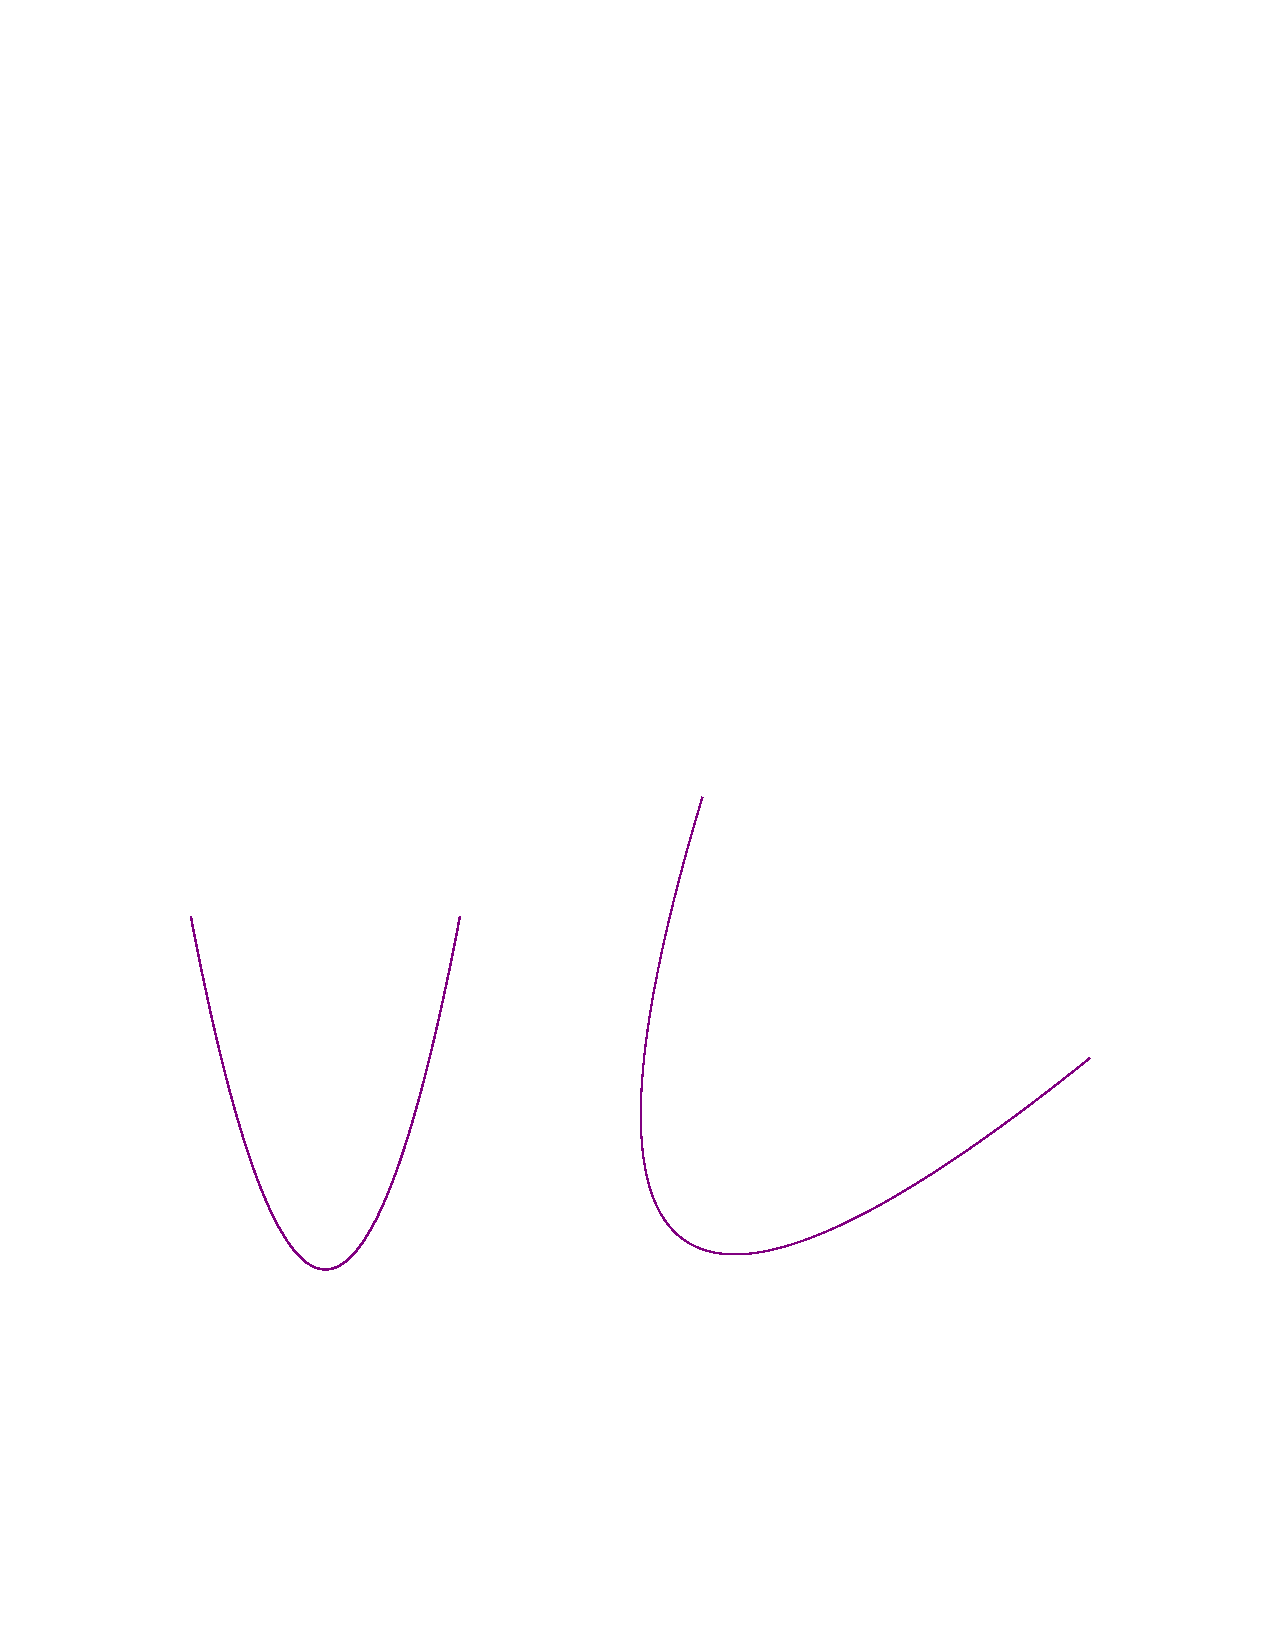
\includegraphics{similarParabolas2}
\end{image}
\vfill

\end{document}
